\documentclass[tikz,border=2pt]{standalone}
\usepackage{amsmath,amssymb}
\usepackage{tikz}
\usetikzlibrary{arrows.meta,matrix}

\begin{document}
% LU decomposition: A = L U with L unit lower triangular (the row-operation multipliers) and
% U upper triangular (the echelon form); solving Ax = b then costs two triangular solves.
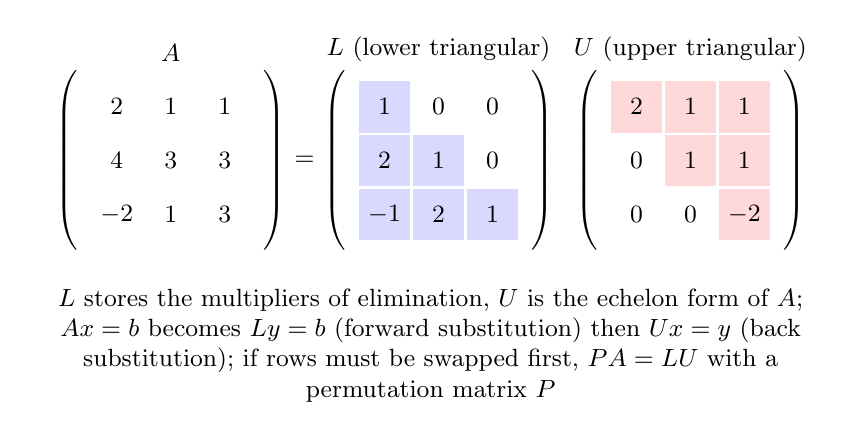
\begin{tikzpicture}[every node/.style={font=\small}]
	\matrix (A) [matrix of math nodes, nodes={minimum size=6.5mm, anchor=center}, left delimiter=(, right delimiter=), column sep=1pt, row sep=1pt] at (0,0) {
		2 & 1 & 1 \\
		4 & 3 & 3 \\
		-2 & 1 & 3 \\
	};
	\node at (1.7,0) {$=$};
	\matrix (L) [matrix of math nodes, nodes={minimum size=6.5mm, anchor=center}, left delimiter=(, right delimiter=), column sep=1pt, row sep=1pt] at (3.4,0) {
		|[fill=blue!15]| 1 & 0 & 0 \\
		|[fill=blue!15]| 2 & |[fill=blue!15]| 1 & 0 \\
		|[fill=blue!15]| -1 & |[fill=blue!15]| 2 & |[fill=blue!15]| 1 \\
	};
	\matrix (U) [matrix of math nodes, nodes={minimum size=6.5mm, anchor=center}, left delimiter=(, right delimiter=), column sep=1pt, row sep=1pt] at (6.6,0) {
		|[fill=red!15]| 2 & |[fill=red!15]| 1 & |[fill=red!15]| 1 \\
		0 & |[fill=red!15]| 1 & |[fill=red!15]| 1 \\
		0 & 0 & |[fill=red!15]| -2 \\
	};
	\node[anchor=south, font=\small] at (A.north) {$A$};
	\node[anchor=south, font=\small] at (L.north) {$L$ (lower triangular)};
	\node[anchor=south, font=\small] at (U.north) {$U$ (upper triangular)};
	\node[anchor=north, align=flush center, text width=10cm] at (3.3,-1.5) {$L$ stores the multipliers of elimination, $U$ is the echelon form of $A$; $Ax=b$ becomes $Ly=b$ (forward substitution) then $Ux=y$ (back substitution); if rows must be swapped first, $PA=LU$ with a permutation matrix $P$};
\end{tikzpicture}
\end{document}
